\newpage

\subsection{Functional specifications}

\begin{figure}[!h]
    \centering
    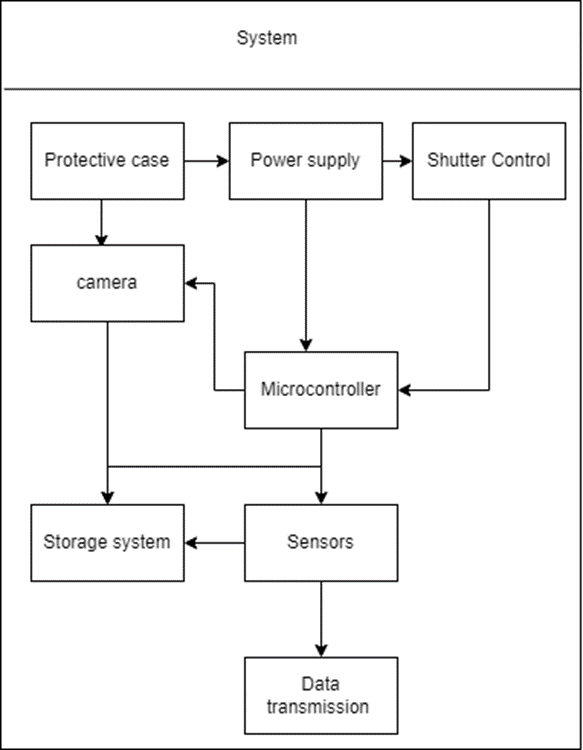
\includegraphics[height=0.5\textheight]{\currfiledir/figures/system.png}
    \caption{Schematic showing different functions interacting inside of the system}
\end{figure}

The diagram illustrates the interconnectivity of these functions, highlighting the relationships and data flow between them. To create a functional system, it is important to ensure that these components are properly integrated and configured to meet the specified technical requirements.

\newpage
\begin{table}[!h]
	\centering
	\begin{tabular}{|c|c|c|c|c|c|}
		\hline
		\rowcolor[HTML]{BFBFBF}
		x                                                  &
		Function                                           &
		Sub-function                                       &
		Criterion                                          &
		Value                                              &
		Flexibility                                          \\ \hline
		F1                                                 &
		\cellcolor[HTML]{CC99FF}Take photos                &
		                                                   &
		                                                   &
		                                                   &
		\cellcolor[HTML]{FFFFFF}{\color[HTML]{FFFFFF} }      \\ \hline
		F1.1                                               &
		                                                   &
		\cellcolor[HTML]{8EA9DB}\begin{tabular}[c]{@{}c@{}}Internal camera \\settings\end{tabular}  &
		                                                   &
		                                                   &
		\\ \hline
		C1.1.1                                             &
		                                                   &
		                                                   &
		\cellcolor[HTML]{A9D08E}Frequency                  &
		\cellcolor[HTML]{FFD966}Once                       &
		\cellcolor[HTML]{ED7D31}2                            \\ \hline
		F1.2                                               &
		                                                   &
		\cellcolor[HTML]{8EA9DB}\begin{tabular}[c]{@{}c@{}}Taking\\ photos regularly\end{tabular}  &
		                                                   &
		                                                   &
		\\ \hline
		C1.2.1                                             &
		                                                   &
		                                                   &
		\cellcolor[HTML]{A9D08E}Frequency                  &
		\cellcolor[HTML]{FFD966}\begin{tabular}[c]{@{}c@{}}2 times a\\ day\end{tabular}  &
		\cellcolor[HTML]{ED7D31}0                            \\ \hline
		F1.3                                               &
		                                                   &
		\cellcolor[HTML]{8EA9DB}\begin{tabular}[c]{@{}c@{}}Taking high-\\ quality photos\end{tabular}  &
		                                                   &
		                                                   &
		\\ \hline
		C1.3.1                                             &
		                                                   &
		                                                   &
		\cellcolor[HTML]{A9D08E}Resolution                 &
		\cellcolor[HTML]{FFD966}1920x1080                    &
		\cellcolor[HTML]{ED7D31}0                            \\ \hline
		C1.3.2                                             &
		                                                   &
		\multicolumn{1}{l|}{}                              &
		\cellcolor[HTML]{A9D08E}Distance                   &
		\cellcolor[HTML]{FFD966}\begin{tabular}[c]{@{}c@{}}300 meters\end{tabular}  &
		\cellcolor[HTML]{ED7D31}0                            \\ \hline
		C1.3.3                                             &
		                                                   &
		\multicolumn{1}{l|}{}                              &
		\cellcolor[HTML]{A9D08E}Fields of view             &
		\cellcolor[HTML]{FFD966}\begin{tabular}[c]{@{}c@{}}32.4°\end{tabular}  &
		\cellcolor[HTML]{ED7D31}1                            \\ \hline 
		F2                                                 &
		\cellcolor[HTML]{CC99FF}\begin{tabular}[c]{@{}c@{}}Possessing an extended\\ battery life\end{tabular}  &
		                                                   &
		                                                   &
		                                                   &
		\\ \hline
		F2.1                                               &
		                                                   &
		\cellcolor[HTML]{8EA9DB}\begin{tabular}[c]{@{}c@{}}Possessing an extended \\battery life\end{tabular}  &
		                                                   &
		                                                   &
		\\ \hline
		C2.1.1                                             &
		                                                   &
		                                                   &
		\cellcolor[HTML]{A9D08E}\begin{tabular}[c]{@{}c@{}}Desired uptime\end{tabular}  &
		\cellcolor[HTML]{FFD966}\(\approx\) 1 year                   &
		\cellcolor[HTML]{ED7D31}1                            \\ \hline
		F3                                                 &
		\cellcolor[HTML]{CC99FF}Storing data               &
		                                                   &
		                                                   &
		                                                   &
		\\ \hline
		F3.1                                               &
		                                                   &
		\cellcolor[HTML]{8EA9DB}Store photos               &
		                                                   &
		                                                   &
		\\ \hline
		C3.1.1                                             &
		                                                   &
		                                                   &
		\cellcolor[HTML]{A9D08E}\begin{tabular}[c]{@{}c@{}}Picture-dedicated \\storage space\end{tabular}  &
		\cellcolor[HTML]{FFD966}\textgreater 16 Go         &
		\cellcolor[HTML]{ED7D31}1                            \\ \hline
		F3.2                                               &
		                                                   &
		\cellcolor[HTML]{8EA9DB}\begin{tabular}[c]{@{}c@{}}Storing  \\ information on \\ the device state\end{tabular} &
		                                                   &
		                                                   &
		\\ \hline
		C3.2.1                                             &
		                                                   &
		                                                   &
		\cellcolor[HTML]{A9D08E}\begin{tabular}[c]{@{}c@{}}Information-dedicated \\ storage  \\ space\end{tabular} &
		\cellcolor[HTML]{FFD966}16 Mo                      &
		\cellcolor[HTML]{ED7D31}3                            \\ \hline
		C3.2.2                                             &
		                                                   &
		                                                   &
		\cellcolor[HTML]{A9D08E}\begin{tabular}[c]{@{}c@{}}Logging period\end{tabular} &
		\cellcolor[HTML]{FFD966}\(\approx\) 1 months                 &
		\cellcolor[HTML]{ED7D31}3                            \\ \hline
		F4                                                 &
		\cellcolor[HTML]{CC99FF}\begin{tabular}[c]{@{}c@{}}Conveying system \\status information\end{tabular} &
		                                                   &
		                                                   &
		                                                   &
		\\ \hline
		F4.1                                               &
		                                                   &
		\cellcolor[HTML]{8EA9DB}Collecting information             &
		                                                   &
		                                                   &
		\\ \hline
		C4.1.1                                             &
		                                                   &
		                                                   &
		\cellcolor[HTML]{A9D08E}\begin{tabular}[c]{@{}c@{}}Remaining battery\\charge percentage\end{tabular} &
		\cellcolor[HTML]{FFD966}\begin{tabular}[c]{@{}c@{}}Error margin \\ of 10\%\end{tabular} &
		\cellcolor[HTML]{ED7D31}2                            \\ \hline
	\end{tabular}
\end{table}

\newpage

% Please add the following required packages to your document preamble:
% \usepackage{multirow}
% \usepackage[table,xcdraw]{xcolor}
% If you use beamer only pass "xcolor=table" option, i.e. \documentclass[xcolor=table]{beamer}
% Please add the following required packages to your document preamble:
% \usepackage{multirow}
% \usepackage[table,xcdraw]{xcolor}
% If you use beamer only pass "xcolor=table" option, i.e. \documentclass[xcolor=table]{beamer}
\begin{table}[!h]
    \centering
    \begin{tabular}{|c|c|c|c|c|c|}
    \hline
     &
       &
       &
      \cellcolor[HTML]{A9D08E} &
      \cellcolor[HTML]{FFD966}\begin{tabular}[c]{@{}c@{}}0°C to 5\\ 0°C\end{tabular} &
      \cellcolor[HTML]{ED7D31}2 \\ \cline{5-6} 
    \multirow{-2}{*}{C4.1.2} &
      \multirow{-2}{*}{} &
      \multirow{-2}{*}{} &
      \multirow{-2}{*}{\cellcolor[HTML]{A9D08E}Temperature} &
      \cellcolor[HTML]{FFD966}\begin{tabular}[c]{@{}c@{}}Precision \\ of 1°C\end{tabular} &
      \cellcolor[HTML]{ED7D31}0 \\ \hline
    C4.1.3 &
       &
       &
      \cellcolor[HTML]{A9D08E}Humidity &
      \cellcolor[HTML]{FFD966}\begin{tabular}[c]{@{}c@{}}80 to \\ 100\%\end{tabular} &
      \cellcolor[HTML]{ED7D31}2 \\ \hline
    C4.1.4 &
       &
       &
      \cellcolor[HTML]{A9D08E}\begin{tabular}[c]{@{}c@{}}Remaining\\  storage\\  space\end{tabular} &
      \cellcolor[HTML]{FFD966}\begin{tabular}[c]{@{}c@{}}Warning \\ at 90\%\end{tabular} &
      \cellcolor[HTML]{ED7D31}2 \\ \hline
    C4.1.5 &
       &
       &
      \cellcolor[HTML]{A9D08E}\begin{tabular}[c]{@{}c@{}}Device \\ motion\end{tabular} &
      \cellcolor[HTML]{FFD966}\begin{tabular}[c]{@{}c@{}}Precision : \\ ± 1cm | \\ ± 1°\end{tabular} &
      \cellcolor[HTML]{ED7D31}1 \\ \hline
    F4.2 &
       &
      \cellcolor[HTML]{8EA9DB}\begin{tabular}[c]{@{}c@{}}Transmitting \\ data remotely\end{tabular} &
       &
       &
       \\ \hline
    C4.2.1 &
       &
       &
      \cellcolor[HTML]{A9D08E}Range &
      \cellcolor[HTML]{FFD966}\(\geq\) 10km &
      \cellcolor[HTML]{ED7D31}1 \\ \hline
    F5 &
      \cellcolor[HTML]{CC99FF}\begin{tabular}[c]{@{}c@{}}Working in a\\  specific \\ environment\end{tabular} &
       &
       &
       &
       \\ \hline
    F5.1 &
       &
      \cellcolor[HTML]{8EA9DB}\begin{tabular}[c]{@{}c@{}}Resisting Central \\ African climate\end{tabular} &
       &
       &
       \\ \hline
    C5.1.1 &
       &
       &
      \cellcolor[HTML]{A9D08E}\begin{tabular}[c]{@{}c@{}}Humidity \\ and fog\end{tabular} &
      \cellcolor[HTML]{FFD966}\begin{tabular}[c]{@{}c@{}}\textgreater 90\% of \\ humidity\end{tabular} &
      \cellcolor[HTML]{ED7D31}0 \\ \hline
    C5.1.2 &
       &
       &
      \cellcolor[HTML]{A9D08E}Temperature &
      \cellcolor[HTML]{FFD966}20°C to 35°C &
      \cellcolor[HTML]{ED7D31}0 \\ \hline
    C5.1.3 &
       &
       &
      \cellcolor[HTML]{A9D08E}Rain &
      \cellcolor[HTML]{FFD966}\begin{tabular}[c]{@{}c@{}}equivalent to\\ IPX4\end{tabular} &
      \cellcolor[HTML]{ED7D31}0 \\ \hline
    \cellcolor[HTML]{FFFFFF}F5.2 &
      \cellcolor[HTML]{FFFFFF} &
      \cellcolor[HTML]{8EA9DB}Size &
       &
       &
       \\ \hline
    \cellcolor[HTML]{FFFFFF}C5.2.1 &
      \cellcolor[HTML]{FFFFFF} &
       &
      \cellcolor[HTML]{A9D08E}Dimensions &
      \cellcolor[HTML]{FFD966}200x300x150 mm &
      \cellcolor[HTML]{ED7D31}2 \\ \hline
    \cellcolor[HTML]{FFFFFF}F5.3 &
      \cellcolor[HTML]{FFFFFF} &
      \cellcolor[HTML]{8EA9DB}Weight &
       &
       &
       \\ \hline
    \cellcolor[HTML]{FFFFFF}C5.3.1 &
      \cellcolor[HTML]{FFFFFF} &
       &
      \cellcolor[HTML]{A9D08E}Mass &
      \cellcolor[HTML]{FFD966}4 kg &
      \cellcolor[HTML]{ED7D31}1 \\ \hline
    \cellcolor[HTML]{FFFFFF}F5.4 &
      \cellcolor[HTML]{FFFFFF} &
      \cellcolor[HTML]{8EA9DB}\begin{tabular}[c]{@{}c@{}}Installation\end{tabular} &
       &
       &
       \\ \hline
    \cellcolor[HTML]{FFFFFF}C5.4.1 &
      \cellcolor[HTML]{FFFFFF} &
       &
      \cellcolor[HTML]{A9D08E}\begin{tabular}[c]{@{}c@{}}Relevant stand \\ or platform\end{tabular} &
      \cellcolor[HTML]{FFD966}??? &
      \cellcolor[HTML]{ED7D31}1 \\ \hline
    \end{tabular}
\end{table}
\tab\tab